\documentclass[11pt,letterpaper]{article}
\usepackage{listings}
\usepackage{graphicx}
\usepackage{subfigure}
\usepackage{geometry}
\geometry{margin=1.3in}
\lstset{basicstyle=\small\ttfamily}
\begin{document}
\title {Visual Interface Project Proposal}
\author {
	Xiuhan Hu \texttt{(xh2234)} \and     
	Wentao Jiang \texttt{(wj2227)}
}
\maketitle


\section{Introduction}
With the development of internet during recent years, the traditional face-to-face education has been extended to online education. And consequently, the exams for online courses faces the fact that we are lacking of ways of distant proctoring the process at economical cost, which may lead to plagiarism and problems with the integrity of academics\cite{c1}. In this project, we are aiming to develop an online proctoring system\cite{c2}, which utilizes normal online webcam to detect suspicious behaviors during online exam process, and provides feedbacks to the online exam providers. 

This project first identifies the problem: currently there is a lack of methods for preventing cheating of online exams with no human labor and of low costs. Then we propose a method to address this issue efficiently: to assist the protection of the academic integrity of online exams, automated proctoring software using computer vision can be implemented. It is considered to be an example of a visual interface as it gathers the visual interface elements including webcam video input, computer vision recognition of number of faces, face features and eye movements and makes judgement based on the automated analysis.


\section{Objectives and Limitations}

We decide to design a program at least capable of:
\begin{itemize}
\item Detecting if the exam taker is taking test together with someone else. The program should find more than one faces appear in the video.
\item Detecting if the exam taker has some other person take the exam for him/her. We need to recognize the face and determine if it is the right person.
\item Detecting if the test taker is gazing at the screen and not peeping outside it. The program will track the direction of user’s sight and alarm when it is outside the screen for a period of time.
\item The test paper window will cover the full screen and the test taker cannot move or resize it. The program resize itself at the beginning of test and will alarm whenever the user try to move or resize it.
\end{itemize}

Whenever the program detect an abnormal behavior of the exam taker, we will mark out that clip of video for our proctor (real person) to further inspect.

To achieve the objectives, we set some restrictions on the problem domain and we assume:

\begin{itemize}
\item The exam taker should have normal facial feature. We probably cannot track the direction of sight for a strabismus patient.
\item The exam taker should not use a draft paper. We cannot determine whether the guy is looking at a book or writing/reading a draft paper.
\item The video input is genuine. If the test taker use some sophisticated skills to hack the camera of the computer and change the video input into a faked one, we obviously cannot know that.
\end{itemize}

There are still some cases that a real world system probably need to deal with, but we probably will not consider for this project due to the limitation of time:

\begin{itemize}
\item We cannot detect if the test taker is talking with someone outside our scope. He/She probably use a Bluetooth phone and it’s very subtle for a proctor to find out even in offline exam.
\item We cannot allow the test taker to do an open book exam because we suppose the person is staring at the computer. However, cheat sheet is ok since we can provide necessary information on screen.
\end{itemize}

\pagebreak
\section{Anticipated methods and results}

There are two major modules in our program: face recognition and gaze detection.

Assuming a test taker have a recorded photo in our database:

\begin{figure}[htb!]
  \centering
    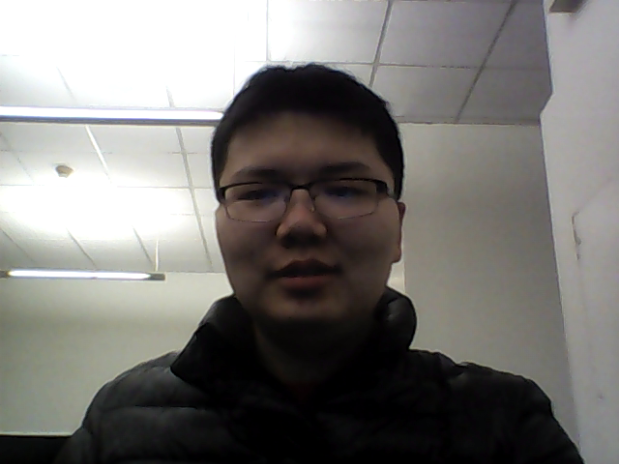
\includegraphics[width=0.35\textwidth]{record}
	\caption{Record in database}
\end{figure}

And here is the normal situation without suspicious behaviors during a exam:

\begin{figure}[htb!]
  \centering
    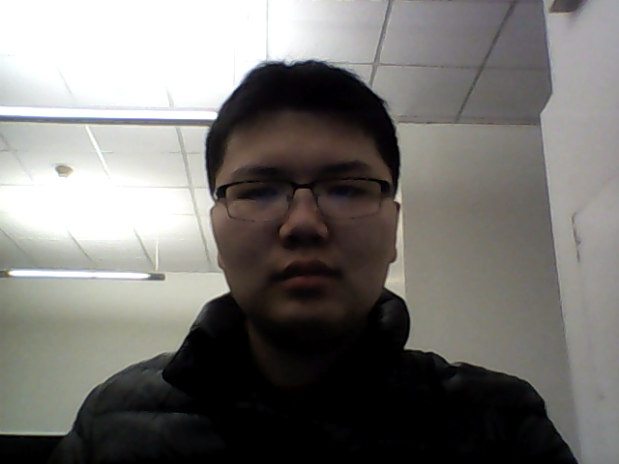
\includegraphics[width=0.35\textwidth]{normal}
	\caption{Normal}
\end{figure}

\subsection{Face recognition}

There are some suspicious situation that require face recognition to figure out.

\begin{figure}[htb!]
  \centering
  \subfigure[Absence]{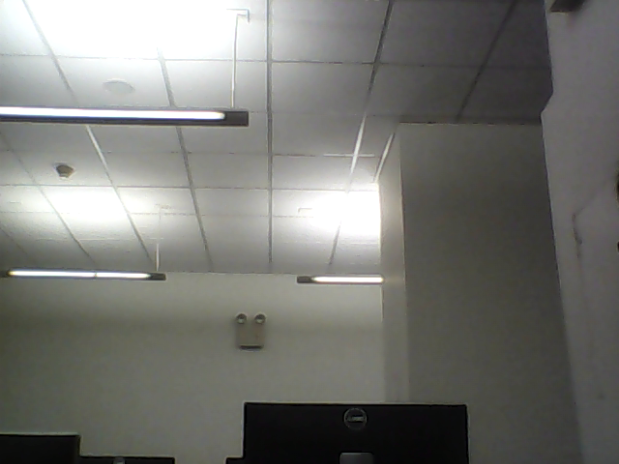
\includegraphics[scale=0.21]{absence}}\quad
  \subfigure[Two Faces]{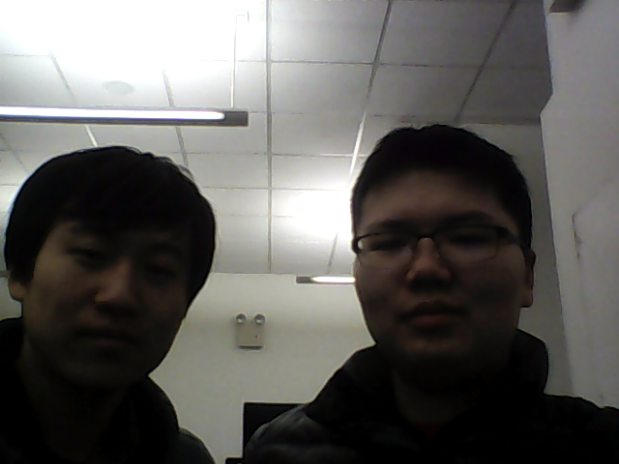
\includegraphics[scale=0.21]{two}}\quad
  \subfigure[Wrong Face]{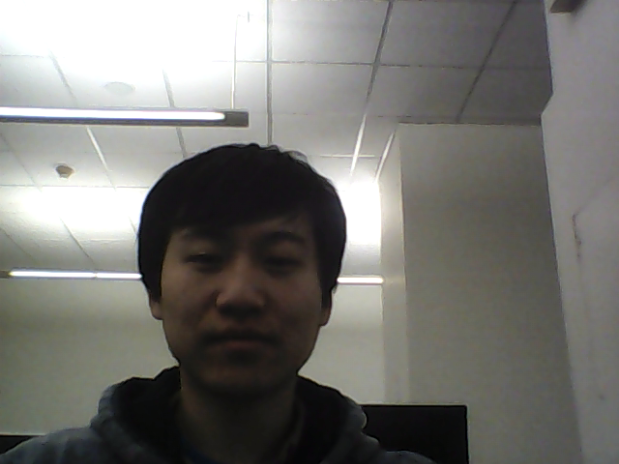
\includegraphics[scale=0.21]{wrong}}
	\caption{Face recognition determined cases}
\end{figure}

We are going to write a simple program to detect the position of a face by implementing a Haar Cascade classifier, and then use a open source sdk, Face++\cite{facepp}, for face recognition.

\subsection{Gaze detection}

Other suspicious situation requires gaze detection to be found out.

\begin{figure}[htb!]
  \centering
  \subfigure[Peep right]{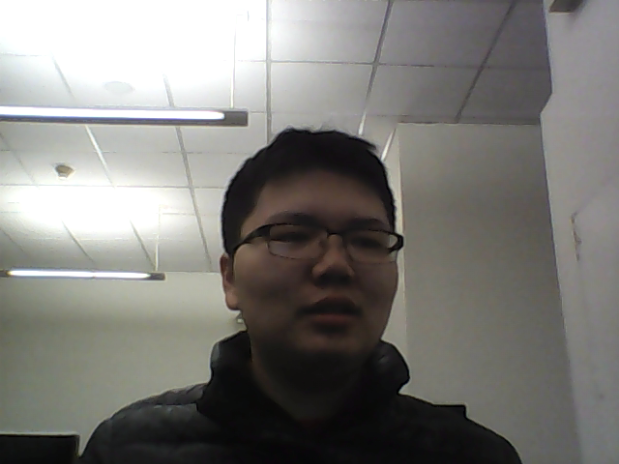
\includegraphics[scale=0.22]{peep1}}\quad
  \subfigure[Peep down]{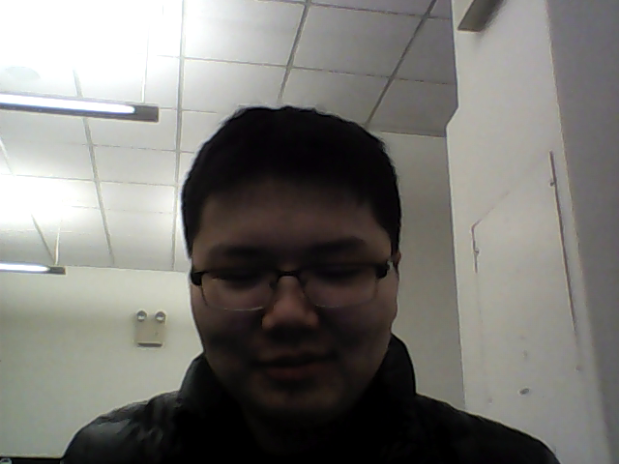
\includegraphics[scale=0.22]{peep2}}
	\caption{Gaze detection determined cases}
\end{figure}

For the detection of gaze, we propose to implement feature-based pupil tracking algorithms from references, which process the images by extracting eye features and make judgement on the direction the eye is looking at\cite{c4,c5}.



\section{Evaluation}

For the evaluation of the proposed system, we can use precision and recall. In general, precision and recall are defined as:
$$precision = TP/(TP+FP)$$
$$recall = TP/(TP+FN)$$
where TP, FP and FN indicates true positive, false positive and false negative respectively. Specifically in our system, the two evaluation factors will be calculated as in figure below. 

\begin{figure}[htb!]
  \centering
    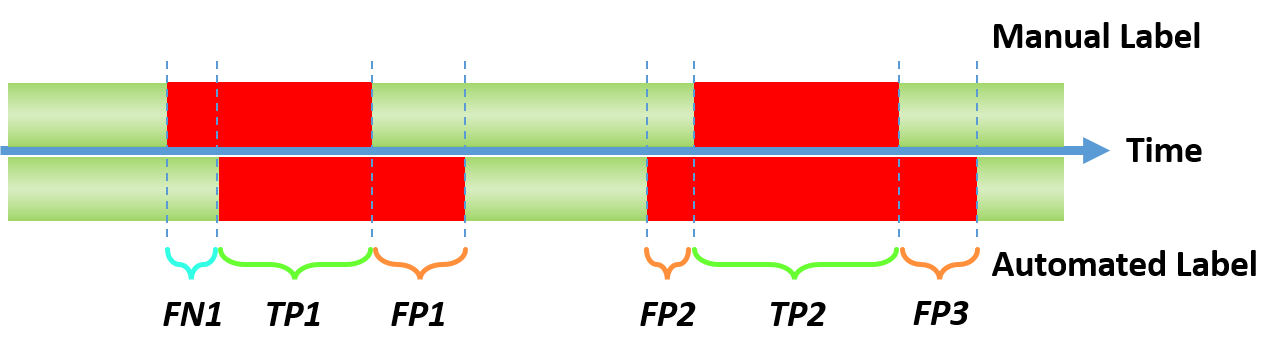
\includegraphics[width=0.8\textwidth]{timeline}
	\caption{evaluation metric definition}
\end{figure}

We first manually label the time windows of a video clip that corresponds to cheating periods, which is taken as true label, and then label the same video clip with the proctoring system. We use the following formulas to calculate precision and recall:
$$precision = \frac{\sum TP}{\sum TP + \sum FP}$$
$$recall = \frac{\sum TP}{\sum TP + \sum FN}$$
where TP is defined as the time windows which are labeled both manually and automatically to be cheating, FP is defined as the time windows which is manually not labeled to be cheating but labeled by the proctoring system to be cheating, and FN is the time windows which is manually labeled to be cheating but missed by the proctoring system. In the figure, the axis is the time of video, and the upper label is from human judgement, while the lower label is the result of the proctoring system. In this particular case we have:
$$precision = \frac{\sum TP}{\sum TP + \sum FP} = \frac{TP1+TP2}{TP1+TP2+FP1+FP2+FP3} $$
$$recall = \frac{\sum TP}{\sum TP + \sum FN} = \frac{TP1+TP2}{TP1+TP2+FN1}$$

Tentatively, we would like to run the evaluation process for 5 to 10 video clips, and collect the precision and recall values. If the result is not satisfactory, we would go back to the step of facial recognition and eye movement detection algorithms and make adjustments.

\section{Teamwork}

As a team of two, we decide to divide the project into following stages sequentially and assign the responsibility evenly.

\begin{enumerate}
\item Modules of program:
\begin{enumerate}
 \item Face detection and recognition: Xiuhan
 \item Gaze detection: Wentao
\end{enumerate}
\item Integration and Interface: Xiuhan
\item Test and experiment: Wentao
\item Report and document: Both
\end{enumerate}

\begin{thebibliography}{9}

\bibitem{c1} Howlett, Bernadette, and Beverly Hewett. "Securing and proctoring online tests." online assessment and measurement: Foundations and challenges(2006): 300-329.
\bibitem{c2} Bedford, D. Wayne, Janie R. Gregg, and M. Suzanne Clinton. "Preventing online cheating with technology: A pilot study of remote proctor and an update of its use." Journal of Higher Education Theory and Practice 11.2 (2011): 41-59.
\bibitem{c4} Timm, Fabian, and Erhardt Barth. "Accurate Eye Centre Localisation by Means of Gradients." VISAPP. 2011.
\bibitem{c5} Smith, Brian A., et al. "Gaze locking: Passive eye contact detection for human-object interaction." Proceedings of the 26th annual ACM symposium on User interface software and technology. ACM, 2013.
\bibitem{facepp} Megvii Inc. Face++ Research Toolkit. www.faceplusplus.com, December 2013.

\end{thebibliography}


\end{document}

